\documentclass[11pt, letterpaper]{article}
\usepackage{color}
\usepackage[linktoc=all]{hyperref}

\usepackage[bindingoffset=0.2in,left=1in,right=1in,top=0.5in,bottom=1in,footskip=.25in]{geometry}
\usepackage{enumitem}
\usepackage{graphicx}
\usepackage{subcaption}
\usepackage{mwe}
\usepackage{parskip}
\usepackage{indentfirst}
\usepackage{textcomp}
\usepackage[formats]{listings}
\usepackage{xcolor}
\definecolor{listinggray}{gray}{0.9}
\definecolor{lbcolor}{rgb}{0.9,0.9,0.9}
\definecolor{Darkgreen}{RGB}{11,100,35}
\usepackage{geometry}

\geometry{
	body={7.0in, 9.8in},
	left=0.75in,
	top=0.6in
}

\hypersetup{
	colorlinks,
	citecolor=black,
	filecolor=black,
	linkcolor=black,
	urlcolor=black
}

\lstdefineformat{Java}{%
\{=\newline\string\newline\indent,%
\}=[;]\newline\noindent\string\newline,%
\};=\newline\noindent\string\newline,%
;=[\ ]\string\space}

\lstset{
	backgroundcolor=\color{lbcolor},
	upquote=true,
	language=Java,
	captionpos=b,
	tabsize = 4, %% Sets tab space width.
	basicstyle = \small \ttfamily , %% Sets listing font and size.
	breaklines = true, %% Enables line breaking.
	numberstyle = \tiny,
	frame=single,
	numbersep=5pt,
	prebreak = \raisebox{0ex}[0ex][0ex]{\ensuremath{\hookleftarrow}},
	basicstyle=\footnotesize,
	identifierstyle=\ttfamily,
	basicstyle=\scriptsize,
	showstringspaces = false, %% Prevents space marking in strings, string is defined as the text that is generally printed directly to the console.
	numbers = left, %% Displays line numbers on the left.
	commentstyle = \color{Darkgreen}, %% Sets comment color.
	keywordstyle = \color{blue}, %% Sets  keyword color.
	stringstyle = \color{red}, %% Sets  string color.
	rulecolor = \color{black}, %% Sets frame color to avoid being affected by text color.
}

\setlength{\parindent}{15pt}
%opening
\title{\textbf{Program 4 Report}}
\author{Yangxiao Wang}
\date{ }



\begin{document}
	
	\maketitle
	
	\tableofcontents
	\pagebreak
	
	\section{Documentation}
	In this project, we are using spark to implement Breadth First Search algorithm. My approach followed the provided descriptions in the assignment PDF. It first read the whole graph into the JavaPairRDD with String and customized object Data. Data contains all the attributes of a vertex. Then I started the while loop with the source vertex active, in the while loop:
	\begin{itemize} 
		\item For every active vertex, update its neighbors' distance to source. 
		\item For every vertex has a new and shorter distance, active this vertex.
	\end{itemize}
	
	\section {Source code}
	\subsection{ShortBFS.java}
	\vspace{-0.2in}
	\begin{lstlisting} [format=Java]
	import org.apache.spark.SparkConf;
	import org.apache.spark.api.java.JavaPairRDD;
	import org.apache.spark.api.java.JavaRDD;
	import org.apache.spark.api.java.JavaSparkContext;
	import scala.Tuple2;
	
	import java.io.Serializable;
	import java.util.ArrayList;
	import java.util.List;
	
	/**
	* @author Yangxiao on 11/20/2018.
	*/
	
	public class ShortBFS {
	
	public static final String ACTIVE = "ACTIVE";
	public static final String INACTIVE = "INACTIVE";
	
	public static void main(String[] args) {
	// start Sparks and read a given input file
	String inputFile = args[0];
	String start = args[1];
	String end = args[2];
	SparkConf conf = new SparkConf().setAppName("BFS-based Shortest Path Search");
	JavaSparkContext jsc = new JavaSparkContext(conf);
	JavaRDD<String> lines = jsc.textFile(inputFile);
	// now start a timer
	long startTime = System.currentTimeMillis();
	JavaPairRDD<String, Data> network =
	lines.mapToPair(line -> {
	int indE = line.indexOf("=");
	String vID = line.substring(0, indE);
	String[] lists = line.substring(indE + 1).split(";");
	int n = lists.length;
	List<Tuple2<String, Integer>> neighbors = new ArrayList<>();
	for (int i = 0; i < n; i++) {
	String[] parts = lists[i].split(",");
	neighbors.add(new Tuple2<>(parts[0], Integer.parseInt(parts[1])));
	}
	Data data1;
	if (vID.equals(start)) {
	data1 = new Data(neighbors, 0, 0, ACTIVE);
	} else {
	data1 = new Data(neighbors, Integer.MAX_VALUE, Integer.MAX_VALUE, INACTIVE);
	}
	return new Tuple2<>(vID, data1);
	});
	System.out.println("Count = " + network.count() + "\n");
	
	while (network.filter(f -> {
	if (f._2.status.equals(ACTIVE)) {
	return true;
	} else {
	return false;
	}
	}).count() > 0) {
	JavaPairRDD<String, Data> propagatedNetwork = network.flatMapToPair(vertex -> {
	// If a vertex is "ACTIVE", create Tuple2( neighbor, new Data() ) for
	// each neighbor where Data should include a new distance to this neighbor.
	// Add each Tuple2 to a list. Dont forget this vertex itself back to the
	// list. Return all the list items.
	List<Tuple2<String, Data>> list = new ArrayList<>();
	list.add(new Tuple2<>(vertex._1,
	new Data(vertex._2.neighbors, vertex._2.distance, vertex._2.prev,
	INACTIVE)));
	if (vertex._2.status.equals(ACTIVE)) {
	for (Tuple2<String, Integer> neighbor : vertex._2.neighbors) {
	list.add(new Tuple2<>(neighbor._1,
	new Data(new ArrayList<>(), (neighbor._2 + vertex._2.distance),
	Integer.MAX_VALUE, INACTIVE)));
	}
	}
	return list.iterator();
	});
	
	network = propagatedNetwork.reduceByKey((k1, k2) -> {
	// For each key, (i.e, each vertex), find the shortest distance and
	// update this vertex Data attribute.
	List<Tuple2<String, Integer>> neighbors =
	k1.neighbors.size() == 0 ? k2.neighbors : k1.neighbors;
	int dis = Math.min(k1.distance, k2.distance);
	int prev = Math.min(k1.prev, k2.prev);
	return new Data(neighbors, dis, prev, INACTIVE);
	});
	
	network = network.mapValues(value -> {
	// If a vertex new distance is shorter than prev, activate this vertex
	// status and replace prev with the new distance.
	if (value.distance < value.prev) {
	return new Data(value.neighbors, value.distance, value.distance, ACTIVE);
	}
	return value;
	});
	}
	List<Data> res = network.lookup(end);
	System.out.println("from " + start + " to " + end + " takes distance = " + res.get(0).distance);
	System.out.println("Time = " + (System.currentTimeMillis() - startTime));
	}
	
	/**
	* Vertex Attributes
	*/
	static class Data implements Serializable {
	List<Tuple2<String, Integer>> neighbors; // <neighbor0, weight0>, ...
	String status; // "INACTIVE" or "ACTIVE"
	Integer distance; // the distance so far from source to this vertex
	Integer prev; // the distance calculated in the previous iteration
	
	public Data() {
	neighbors = new ArrayList<>();
	status = "INACTIVE";
	distance = 0;
	}
	
	public Data(List<Tuple2<String, Integer>> neighbors,
	Integer dist, Integer prev, String status) {
	if (neighbors != null) {
	this.neighbors = new ArrayList<>(neighbors);
	} else {
	this.neighbors = new ArrayList<>();
	}
	this.distance = dist;
	this.prev = prev;
	this.status = status;
	}
	}
	}
	\end{lstlisting}
	\pagebreak
	
	
	\section {Execution output}

	\subsection{Output}
	
	\begin{figure}[h]
		\centering
		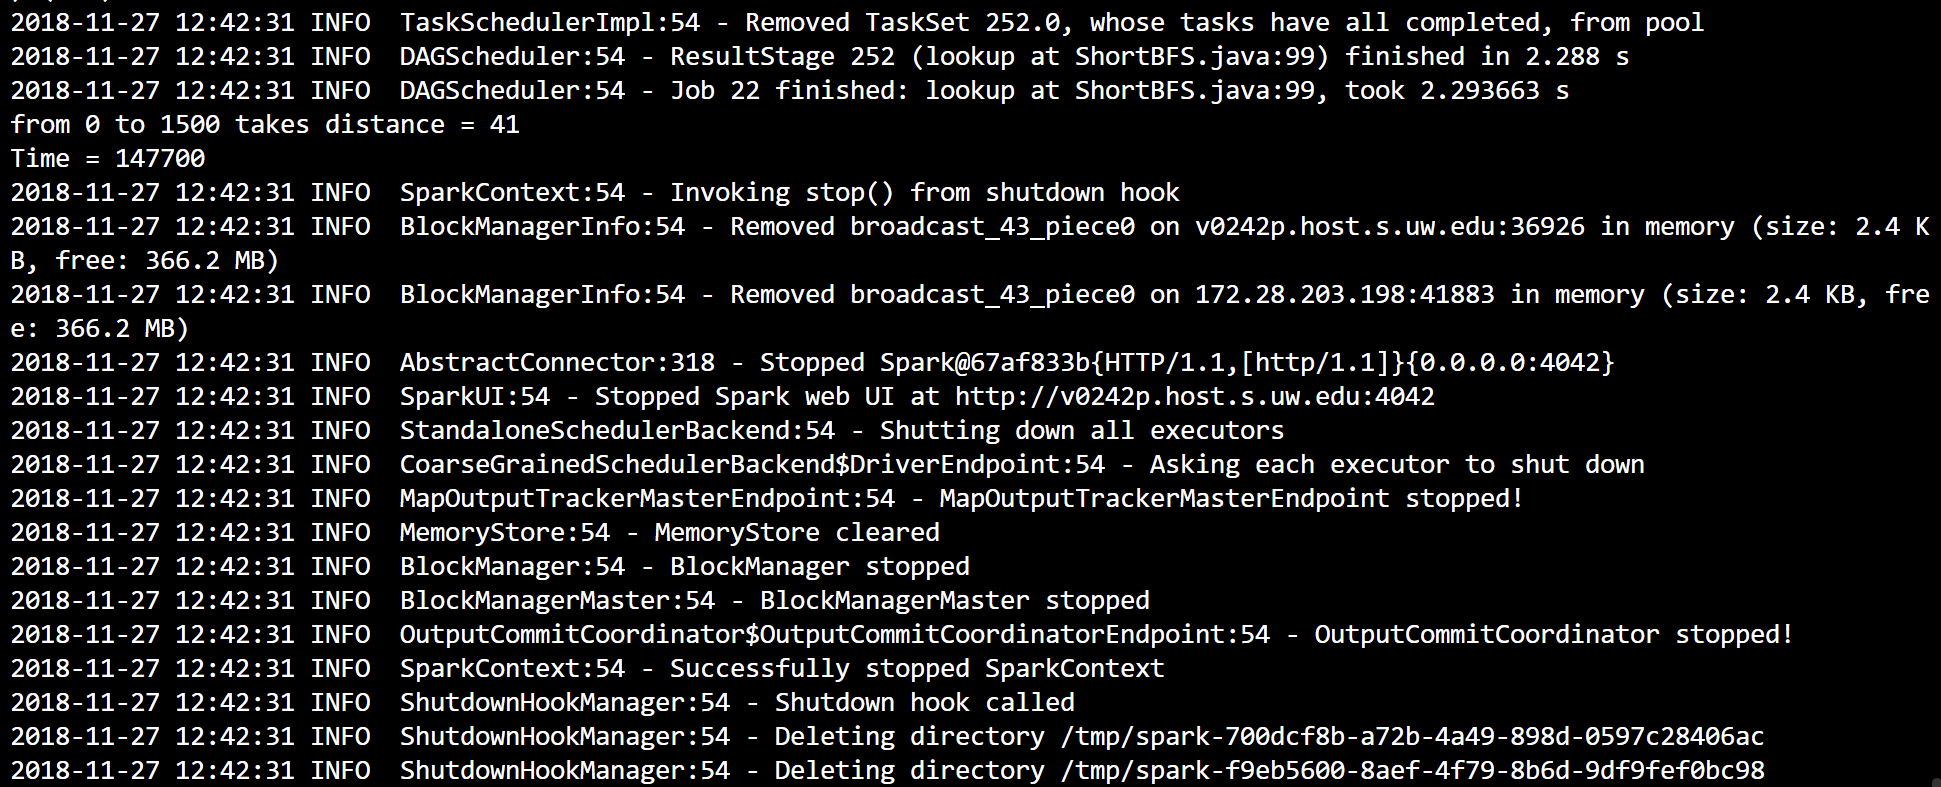
\includegraphics[width=0.7\textwidth]{1500}
		\caption{0-1500}
	\end{figure}

	\begin{figure}[h]
		\centering
		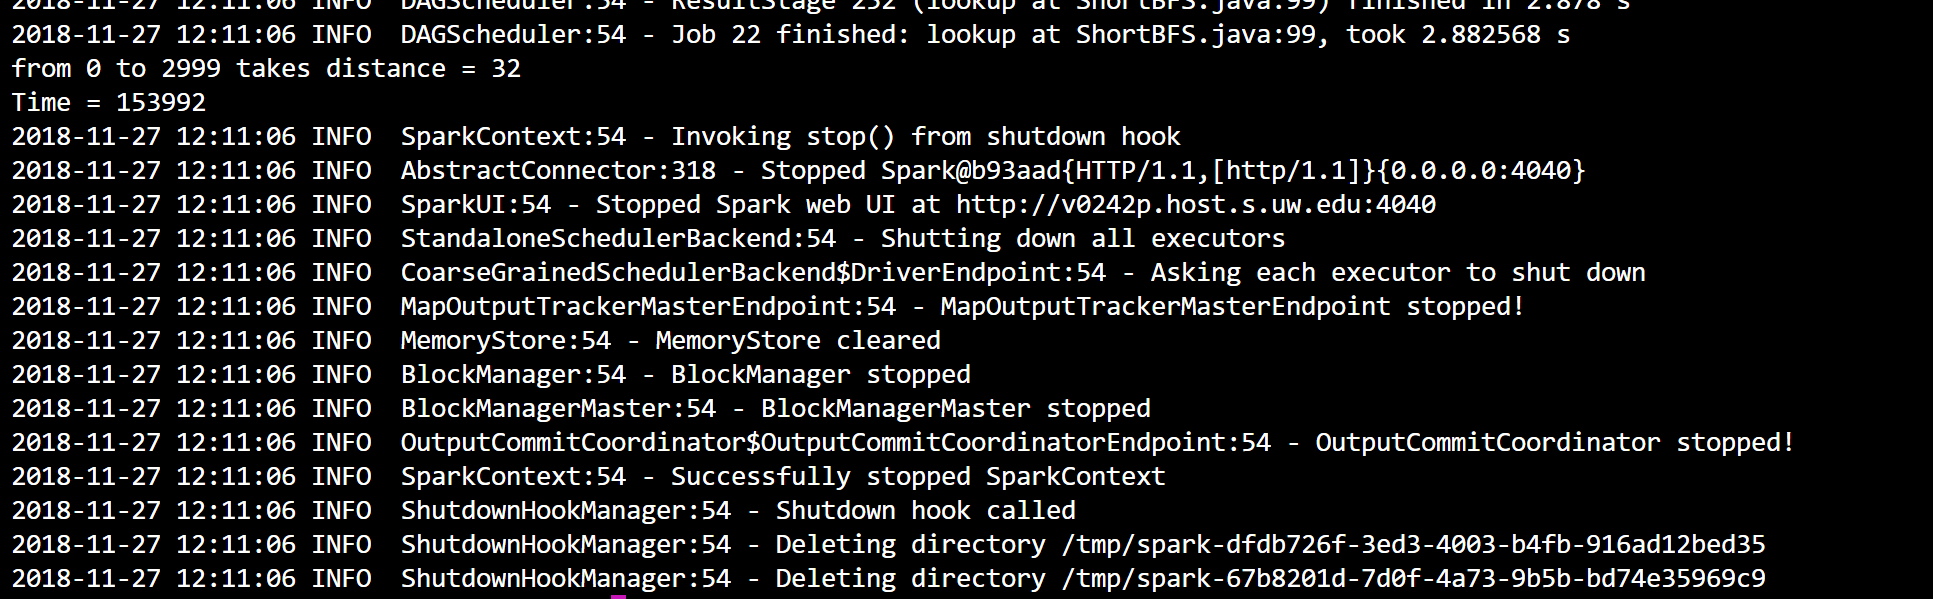
\includegraphics[width=0.7\textwidth]{2999}
		\caption{0-2999 with 12 cores}
	\end{figure}

	\begin{figure}[h]
		\centering
		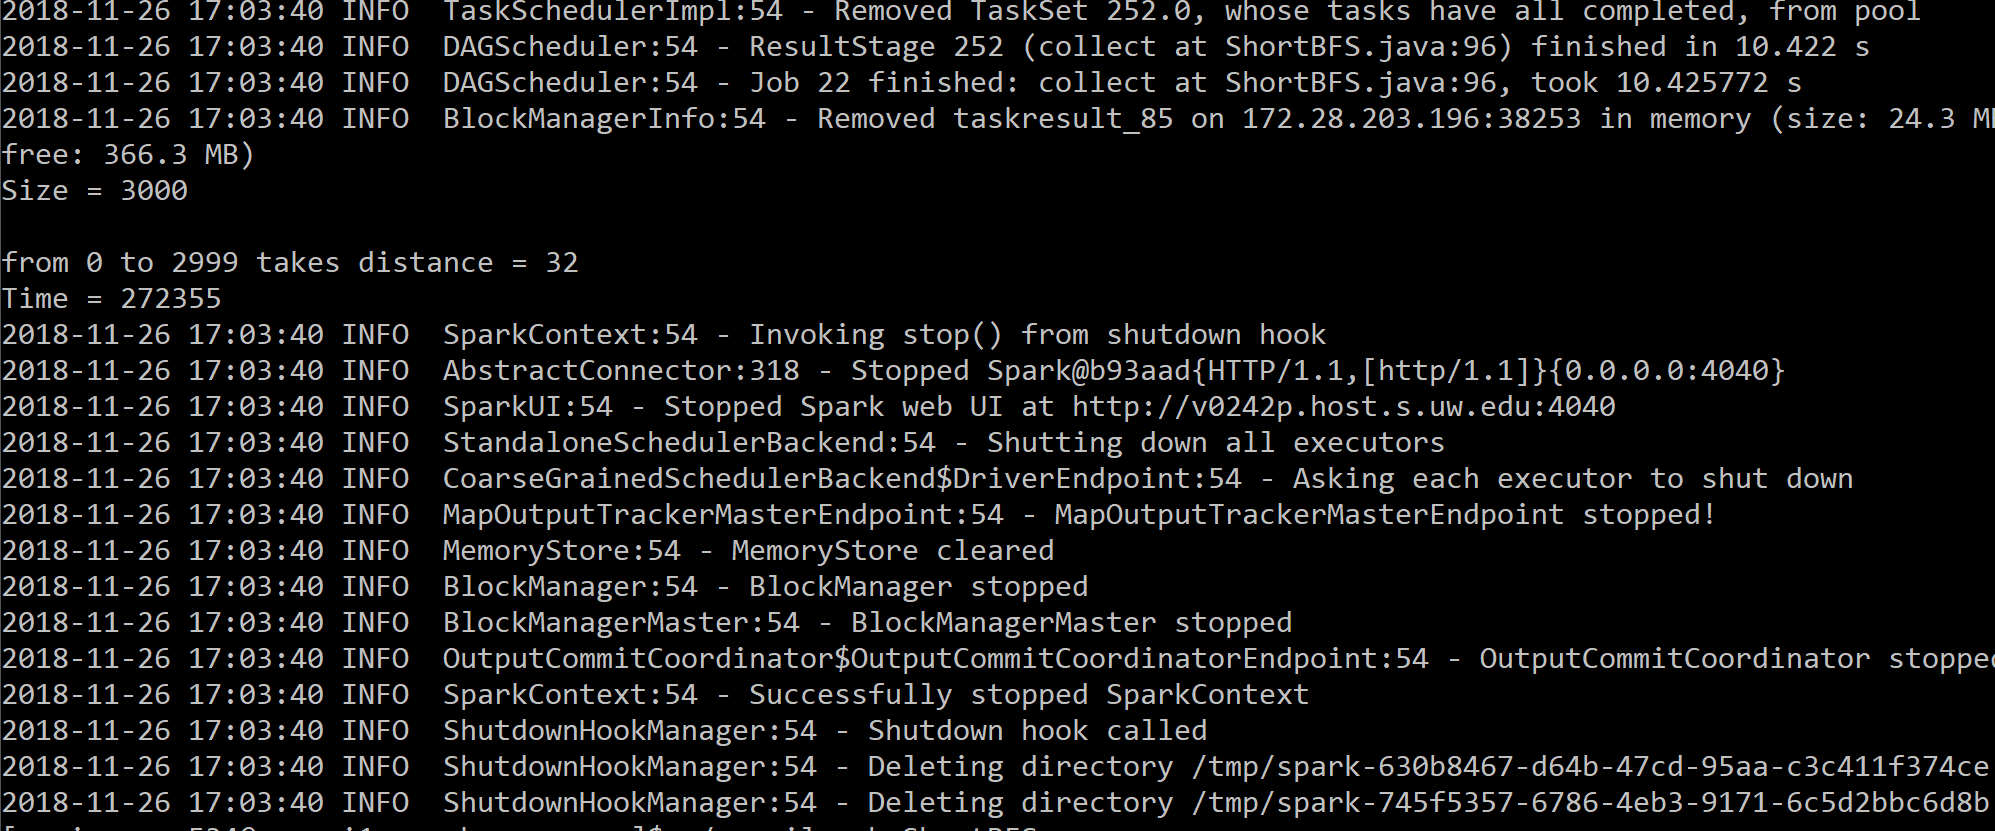
\includegraphics[width=0.7\textwidth]{1core}
		\caption{0-2999 with 1 core}
	\end{figure}
	
	\begin{table}[]
		\centering
		\begin{tabular}{|c|c|c|c|c|}
			\hline
			\# of Comp nodes & \begin{tabular}[c]{@{}l@{}}Avg \# of cores per\\   node\end{tabular} & Total \# of cores & \begin{tabular}[c]{@{}l@{}}Elapsed\\   time (sec)\end{tabular} & \begin{tabular}[c]{@{}l@{}}Performance\\   improvement\end{tabular} \\
			\hline			
			1 & 1 & 1 & 272.355 & 1 \\
			\hline
			1 & 2 & 2 & 221.677 & 1.228612 \\
			\hline
			1 & 3 & 3 & 234.051 & 1.163657 \\
			\hline
			2 & 1 & 2 & 162.512 & 1.675907 \\
			\hline
			2 & 2 & 4 & 192.527 & 1.414633 \\
			\hline
			2 & 3 & 6 & 171.951 & 1.583911 \\
			\hline
			4 & 1 & 4 & 163.253 & 1.6683 \\
			\hline
			4 & 2 & 8 & 197.543 & 1.378712 \\
			\hline
			\textcolor{red}{\textbf{4}} & \textcolor{red}{\textbf{3}} & \textcolor{red}{\textbf{12}} & \textcolor{red}{\textbf{147.7}} & \textcolor{red}{\textbf{1.843974272}} \\
			\hline
		\end{tabular}
	\end{table}
	
	\pagebreak
	
	\section {Discussions}
	
	\begin{itemize} 
		\item Programmability Pros: the original algorithm is easy to implement, it first transfer input file to JavaPairRDD with String and Data. Then it find Active nodes' neighbors, and calculate the distance. And update its distance. These processes are straightforward and easy to implemented. Furthermore, the data exchanging and parallel part are already taken cared by Spark, unlike MPI, I do not need write code for them. \par
		\item Programmability Cons: The Data object is not optimized for this BFS search, and spark api is just generally not easy to understand such as the $flatMapTopair$ and $reduceByKey$.\par
		\item Execution performance Pros: In general, the most time consuming part in Spark is collect operation. Fortunately, my code does not have any collect operations so the performance should be fast with the RDD transformation operations. \par
		\item Execution performance Cons: The RDD transformation processes contain duplicated loops which could slow the execution performance. For example, $network$ to $propagatedNetwork$ with traversal through all items in network, then $propagatedNetwork$ reduced to $network$ with traversal through duplicated items in propagatedNetwork, and loop through network to update distance. To improve this procedure, the updating part can be moved into the reduce part, since only reduced item has updated distance.\par
		
		\item Improvement:
		\begin{lstlisting} [format=Java]
		network = propagatedNetwork.reduceByKey((k1, k2) -> {
		// For each key, (i.e, each vertex), find the shortest distance and
		// update this vertex Data attribute.
		List<Tuple2<String, Integer>> neighbors =
		k1.neighbors.size() == 0 ? k2.neighbors : k1.neighbors;
		int dis = Math.min(k1.distance, k2.distance);
		int prev = Math.min(k1.prev, k2.prev);
		
		String status = (k1.status.equals(ACTIVE) || k2.status.equals(ACTIVE)) ? ACTIVE : INACTIVE;
		
		if (dis < prev || status.equals(ACTIVE)) {
		return new Data(neighbors, dis, dis, ACTIVE);
		} else {
		return new Data(neighbors, dis, prev, INACTIVE);
		}
		});
		\end{lstlisting}
		Check and update the distance while reducing the duplicated keys might improve the performance.
		
	\end{itemize}
		
	
	\section {Lab Sessions 4}
	
	\subsection{Lab4A}
	\begin{lstlisting} [format=Java]
	import org.apache.spark.SparkConf;
	import org.apache.spark.api.java.JavaRDD;
	import org.apache.spark.api.java.JavaSparkContext;
	
	import java.io.Serializable;
	import java.util.Arrays;
	import java.util.Comparator;
	
	public class MyClass {
	public static void main(String[] args) { // a driver program
	// initialize Spark Context
	SparkConf conf = new SparkConf().setAppName("My Driver");
	JavaSparkContext sc = new JavaSparkContext(conf);
	
	// read data from a file
	JavaRDD<String> document = sc.textFile("sample.txt");
	// read data from another data structure
	JavaRDD<Integer> numbers = sc.parallelize(Arrays.asList(0, 1, 2, 3, 4, 5));
	
	// apply tranformations/actions to RDD
	System.out.println("#words = " +
	document.flatMap(s -> Arrays.asList(s.split(" ")).iterator()).count());
	System.out.println("max = " + numbers.max(new MyClassMax()));
	
	sc.stop(); // stop Spark Context
	}
	}
	
	class MyClassMax implements Serializable, Comparator<Integer> {
	@Override
	public int compare(Integer o1, Integer o2) {
	return Integer.compare(o1, o2);
	}
	}
	\end{lstlisting}
	
	\subsection{Lab4A Output}
	\noindent \#words = 11 \newline
	max = 5
	\begin{lstlisting}
	[wyxiao_css534@cssmpi1 spark_programs]$ spark-submit --class MyClass --master local MyClass.jar
	2018-11-21 20:14:02 WARN  NativeCodeLoader:62 - Unable to load native-hadoop library for your platform... using builtin-java classes where applicable
	2018-11-21 20:14:02 INFO  SparkContext:54 - Running Spark version 2.3.1
	2018-11-21 20:14:02 INFO  SparkContext:54 - Submitted application: My Driver
	2018-11-21 20:14:02 INFO  SecurityManager:54 - Changing view acls to: wyxiao_css534
	2018-11-21 20:14:02 INFO  SecurityManager:54 - Changing modify acls to: wyxiao_css534
	2018-11-21 20:14:02 INFO  SecurityManager:54 - Changing view acls groups to:
	2018-11-21 20:14:02 INFO  SecurityManager:54 - Changing modify acls groups to:
	2018-11-21 20:14:02 INFO  SecurityManager:54 - SecurityManager: authentication disabled; ui acls disabled; users  with view permissions: Set(wyxiao_css534); groups with view permissions: Set(); users  with modify permissions: Set(wyxiao_css534); groups with modify permissions: Set()
	2018-11-21 20:14:03 INFO  Utils:54 - Successfully started service 'sparkDriver' on port 33246.
	2018-11-21 20:14:03 INFO  SparkEnv:54 - Registering MapOutputTracker
	2018-11-21 20:14:03 INFO  SparkEnv:54 - Registering BlockManagerMaster
	2018-11-21 20:14:03 INFO  BlockManagerMasterEndpoint:54 - Using org.apache.spark.storage.DefaultTopologyMapper for getting topology information
	2018-11-21 20:14:03 INFO  BlockManagerMasterEndpoint:54 - BlockManagerMasterEndpoint up
	2018-11-21 20:14:03 INFO  DiskBlockManager:54 - Created local directory at /tmp/blockmgr-887fd971-00d2-43b5-afd9-ad8826788558
	2018-11-21 20:14:03 INFO  MemoryStore:54 - MemoryStore started with capacity 366.3 MB
	2018-11-21 20:14:03 INFO  SparkEnv:54 - Registering OutputCommitCoordinator
	2018-11-21 20:14:03 INFO  log:192 - Logging initialized @1672ms
	2018-11-21 20:14:03 INFO  Server:346 - jetty-9.3.z-SNAPSHOT
	2018-11-21 20:14:03 INFO  Server:414 - Started @1749ms
	2018-11-21 20:14:03 INFO  AbstractConnector:278 - Started ServerConnector@5dda6f9{HTTP/1.1,[http/1.1]}{0.0.0.0:4040}
	2018-11-21 20:14:03 INFO  Utils:54 - Successfully started service 'SparkUI' on port 4040.
	2018-11-21 20:14:03 INFO  ContextHandler:781 - Started o.s.j.s.ServletContextHandler@6bc28a83{/jobs,null,AVAILABLE,@Spark}2018-11-21 20:14:03 INFO  ContextHandler:781 - Started o.s.j.s.ServletContextHandler@384fc774{/jobs/json,null,AVAILABLE,@Spark}
	2018-11-21 20:14:03 INFO  ContextHandler:781 - Started o.s.j.s.ServletContextHandler@e3cee7b{/jobs/job,null,AVAILABLE,@Spark}
	2018-11-21 20:14:03 INFO  ContextHandler:781 - Started o.s.j.s.ServletContextHandler@6b9267b{/jobs/job/json,null,AVAILABLE,@Spark}
	2018-11-21 20:14:03 INFO  ContextHandler:781 - Started o.s.j.s.ServletContextHandler@408b35bf{/stages,null,AVAILABLE,@Spark}
	2018-11-21 20:14:03 INFO  ContextHandler:781 - Started o.s.j.s.ServletContextHandler@29ad44e3{/stages/json,null,AVAILABLE,@Spark}
	2018-11-21 20:14:03 INFO  ContextHandler:781 - Started o.s.j.s.ServletContextHandler@15bcf458{/stages/stage,null,AVAILABLE,@Spark}
	2018-11-21 20:14:03 INFO  ContextHandler:781 - Started o.s.j.s.ServletContextHandler@fac80{/stages/stage/json,null,AVAILABLE,@Spark}
	2018-11-21 20:14:03 INFO  ContextHandler:781 - Started o.s.j.s.ServletContextHandler@726386ed{/stages/pool,null,AVAILABLE,@Spark}
	2018-11-21 20:14:03 INFO  ContextHandler:781 - Started o.s.j.s.ServletContextHandler@649f2009{/stages/pool/json,null,AVAILABLE,@Spark}
	2018-11-21 20:14:03 INFO  ContextHandler:781 - Started o.s.j.s.ServletContextHandler@14bb2297{/storage,null,AVAILABLE,@Spark}
	2018-11-21 20:14:03 INFO  ContextHandler:781 - Started o.s.j.s.ServletContextHandler@69adf72c{/storage/json,null,AVAILABLE,@Spark}
	2018-11-21 20:14:03 INFO  ContextHandler:781 - Started o.s.j.s.ServletContextHandler@797501a{/storage/rdd,null,AVAILABLE,@Spark}
	2018-11-21 20:14:03 INFO  ContextHandler:781 - Started o.s.j.s.ServletContextHandler@1a15b789{/storage/rdd/json,null,AVAILABLE,@Spark}
	2018-11-21 20:14:03 INFO  ContextHandler:781 - Started o.s.j.s.ServletContextHandler@57f791c6{/environment,null,AVAILABLE,@Spark}
	2018-11-21 20:14:03 INFO  ContextHandler:781 - Started o.s.j.s.ServletContextHandler@51650883{/environment/json,null,AVAILABLE,@Spark}
	2018-11-21 20:14:03 INFO  ContextHandler:781 - Started o.s.j.s.ServletContextHandler@6c4f9535{/executors,null,AVAILABLE,@Spark}
	2018-11-21 20:14:03 INFO  ContextHandler:781 - Started o.s.j.s.ServletContextHandler@5bd1ceca{/executors/json,null,AVAILABLE,@Spark}
	2018-11-21 20:14:03 INFO  ContextHandler:781 - Started o.s.j.s.ServletContextHandler@30c31dd7{/executors/threadDump,null,AVAILABLE,@Spark}
	2018-11-21 20:14:03 INFO  ContextHandler:781 - Started o.s.j.s.ServletContextHandler@499b2a5c{/executors/threadDump/json,null,AVAILABLE,@Spark}
	2018-11-21 20:14:03 INFO  ContextHandler:781 - Started o.s.j.s.ServletContextHandler@596df867{/static,null,AVAILABLE,@Spark}
	2018-11-21 20:14:03 INFO  ContextHandler:781 - Started o.s.j.s.ServletContextHandler@3e587920{/,null,AVAILABLE,@Spark}
	2018-11-21 20:14:03 INFO  ContextHandler:781 - Started o.s.j.s.ServletContextHandler@2ef8a8c3{/api,null,AVAILABLE,@Spark} 2018-11-21 20:14:03 INFO  ContextHandler:781 - Started o.s.j.s.ServletContextHandler@7544a1e4{/jobs/job/kill,null,AVAILABLE,@Spark}
	2018-11-21 20:14:03 INFO  ContextHandler:781 - Started o.s.j.s.ServletContextHandler@70e0accd{/stages/stage/kill,null,AVAILABLE,@Spark}
	2018-11-21 20:14:03 INFO  SparkUI:54 - Bound SparkUI to 0.0.0.0, and started at http://v0242p.host.s.uw.edu:4040
	2018-11-21 20:14:03 INFO  SparkContext:54 - Added JAR file:/home/wyxiao_css534/spark_programs/MyClass.jar at spark://v0242p.host.s.uw.edu:33246/jars/MyClass.jar with timestamp 1542860043497
	2018-11-21 20:14:03 INFO  Executor:54 - Starting executor ID driver on host localhost
	2018-11-21 20:14:03 INFO  Utils:54 - Successfully started service 'org.apache.spark.network.netty.NettyBlockTransferService' on port 41795.
	2018-11-21 20:14:03 INFO  NettyBlockTransferService:54 - Server created on v0242p.host.s.uw.edu:41795
	2018-11-21 20:14:03 INFO  BlockManager:54 - Using org.apache.spark.storage.RandomBlockReplicationPolicy for block replication policy
	2018-11-21 20:14:03 INFO  BlockManagerMaster:54 - Registering BlockManager BlockManagerId(driver, v0242p.host.s.uw.edu, 41795, None)
	2018-11-21 20:14:03 INFO  BlockManagerMasterEndpoint:54 - Registering block manager v0242p.host.s.uw.edu:41795 with 366.3 MB RAM, BlockManagerId(driver, v0242p.host.s.uw.edu, 41795, None)
	2018-11-21 20:14:03 INFO  BlockManagerMaster:54 - Registered BlockManager BlockManagerId(driver, v0242p.host.s.uw.edu, 41795, None)
	2018-11-21 20:14:03 INFO  BlockManager:54 - Initialized BlockManager: BlockManagerId(driver, v0242p.host.s.uw.edu, 41795, None)
	2018-11-21 20:14:03 INFO  ContextHandler:781 - Started o.s.j.s.ServletContextHandler@6ce90bc5{/metrics/json,null,AVAILABLE,@Spark}
	2018-11-21 20:14:04 INFO  MemoryStore:54 - Block broadcast_0 stored as values in memory (estimated size 236.7 KB, free 366.1 MB)
	2018-11-21 20:14:04 INFO  MemoryStore:54 - Block broadcast_0_piece0 stored as bytes in memory (estimated size 22.9 KB, free 366.0 MB)
	2018-11-21 20:14:04 INFO  BlockManagerInfo:54 - Added broadcast_0_piece0 in memory on v0242p.host.s.uw.edu:41795 (size: 22.9 KB, free: 366.3 MB)
	2018-11-21 20:14:04 INFO  SparkContext:54 - Created broadcast 0 from textFile at MyClass.java:20
	2018-11-21 20:14:04 INFO  FileInputFormat:249 - Total input paths to process : 1
	2018-11-21 20:14:04 INFO  SparkContext:54 - Starting job: count at MyClass.java:26
	2018-11-21 20:14:04 INFO  DAGScheduler:54 - Got job 0 (count at MyClass.java:26) with 1 output partitions
	2018-11-21 20:14:04 INFO  DAGScheduler:54 - Final stage: ResultStage 0 (count at MyClass.java:26)
	2018-11-21 20:14:04 INFO  DAGScheduler:54 - Parents of final stage: List()
	2018-11-21 20:14:04 INFO  DAGScheduler:54 - Missing parents: List()
	2018-11-21 20:14:04 INFO  DAGScheduler:54 - Submitting ResultStage 0 (MapPartitionsRDD[3] at flatMap at MyClass.java:26), which has no missing parents
	2018-11-21 20:14:04 INFO  MemoryStore:54 - Block broadcast_1 stored as values in memory (estimated size 4.3 KB, free 366.0 MB)
	2018-11-21 20:14:04 INFO  MemoryStore:54 - Block broadcast_1_piece0 stored as bytes in memory (estimated size 2.5 KB, free 366.0 MB)
	2018-11-21 20:14:04 INFO  BlockManagerInfo:54 - Added broadcast_1_piece0 in memory on v0242p.host.s.uw.edu:41795 (size: 2.5 KB, free: 366.3 MB)
	2018-11-21 20:14:04 INFO  SparkContext:54 - Created broadcast 1 from broadcast at DAGScheduler.scala:1039
	2018-11-21 20:14:04 INFO  DAGScheduler:54 - Submitting 1 missing tasks from ResultStage 0 (MapPartitionsRDD[3] at flatMap at MyClass.java:26) (first 15 tasks are for partitions Vector(0))
	2018-11-21 20:14:04 INFO  TaskSchedulerImpl:54 - Adding task set 0.0 with 1 tasks
	2018-11-21 20:14:04 INFO  TaskSetManager:54 - Starting task 0.0 in stage 0.0 (TID 0, localhost, executor driver, partition 0, PROCESS_LOCAL, 7897 bytes)
	2018-11-21 20:14:04 INFO  Executor:54 - Running task 0.0 in stage 0.0 (TID 0)
	2018-11-21 20:14:04 INFO  Executor:54 - Fetching spark://v0242p.host.s.uw.edu:33246/jars/MyClass.jar with timestamp 1542860043497
	2018-11-21 20:14:04 INFO  TransportClientFactory:267 - Successfully created connection to v0242p.host.s.uw.edu/172.28.203.196:33246 after 25 ms (0 ms spent in bootstraps)
	2018-11-21 20:14:04 INFO  Utils:54 - Fetching spark://v0242p.host.s.uw.edu:33246/jars/MyClass.jar to /tmp/spark-9f7bf541-b76b-4c3c-b7f3-a2e1e79d1f56/userFiles-0a84da4c-a028-481b-8821-9493efcb083e/fetchFileTemp1534358842930517119.tmp
	2018-11-21 20:14:04 INFO  Executor:54 - Adding file:/tmp/spark-9f7bf541-b76b-4c3c-b7f3-a2e1e79d1f56/userFiles-0a84da4c-a028-481b-8821-9493efcb083e/MyClass.jar to class loader
	2018-11-21 20:14:04 INFO  HadoopRDD:54 - Input split: file:/home/wyxiao_css534/spark_programs/sample.txt:0+66
	2018-11-21 20:14:04 INFO  Executor:54 - Finished task 0.0 in stage 0.0 (TID 0). 875 bytes result sent to driver
	2018-11-21 20:14:04 INFO  TaskSetManager:54 - Finished task 0.0 in stage 0.0 (TID 0) in 216 ms on localhost (executor driver) (1/1)
	2018-11-21 20:14:04 INFO  TaskSchedulerImpl:54 - Removed TaskSet 0.0, whose tasks have all completed, from pool
	2018-11-21 20:14:04 INFO  DAGScheduler:54 - ResultStage 0 (count at MyClass.java:26) finished in 0.309 s
	2018-11-21 20:14:04 INFO  DAGScheduler:54 - Job 0 finished: count at MyClass.java:26, took 0.358323 s
	#words = 11
	2018-11-21 20:14:04 INFO  SparkContext:54 - Starting job: max at MyClass.java:27
	2018-11-21 20:14:04 INFO  DAGScheduler:54 - Got job 1 (max at MyClass.java:27) with 1 output partitions
	2018-11-21 20:14:04 INFO  DAGScheduler:54 - Final stage: ResultStage 1 (max at MyClass.java:27)
	2018-11-21 20:14:04 INFO  DAGScheduler:54 - Parents of final stage: List()
	2018-11-21 20:14:04 INFO  DAGScheduler:54 - Missing parents: List()
	2018-11-21 20:14:04 INFO  DAGScheduler:54 - Submitting ResultStage 1 (ParallelCollectionRDD[2] at parallelize at MyClass.java:22), which has no missing parents
	2018-11-21 20:14:04 INFO  MemoryStore:54 - Block broadcast_2 stored as values in memory (estimated size 1864.0 B, free 366.0 MB)
	2018-11-21 20:14:04 INFO  MemoryStore:54 - Block broadcast_2_piece0 stored as bytes in memory (estimated size 1236.0 B, free 366.0 MB)
	2018-11-21 20:14:04 INFO  BlockManagerInfo:54 - Added broadcast_2_piece0 in memory on v0242p.host.s.uw.edu:41795 (size: 1236.0 B, free: 366.3 MB)
	2018-11-21 20:14:04 INFO  SparkContext:54 - Created broadcast 2 from broadcast at DAGScheduler.scala:1039
	2018-11-21 20:14:04 INFO  DAGScheduler:54 - Submitting 1 missing tasks from ResultStage 1 (ParallelCollectionRDD[2] at parallelize at MyClass.java:22) (first 15 tasks are for partitions Vector(0))
	2018-11-21 20:14:04 INFO  TaskSchedulerImpl:54 - Adding task set 1.0 with 1 tasks
	2018-11-21 20:14:04 INFO  TaskSetManager:54 - Starting task 0.0 in stage 1.0 (TID 1, localhost, executor driver, partition 0, PROCESS_LOCAL, 7910 bytes)
	2018-11-21 20:14:04 INFO  Executor:54 - Running task 0.0 in stage 1.0 (TID 1)
	2018-11-21 20:14:04 INFO  Executor:54 - Finished task 0.0 in stage 1.0 (TID 1). 824 bytes result sent to driver
	2018-11-21 20:14:04 INFO  TaskSetManager:54 - Finished task 0.0 in stage 1.0 (TID 1) in 16 ms on localhost (executor driver) (1/1)
	2018-11-21 20:14:04 INFO  TaskSchedulerImpl:54 - Removed TaskSet 1.0, whose tasks have all completed, from pool
	2018-11-21 20:14:04 INFO  DAGScheduler:54 - ResultStage 1 (max at MyClass.java:27) finished in 0.025 s
	2018-11-21 20:14:04 INFO  DAGScheduler:54 - Job 1 finished: max at MyClass.java:27, took 0.028227 s
	max = 5
	2018-11-21 20:14:04 INFO  AbstractConnector:318 - Stopped Spark@5dda6f9{HTTP/1.1,[http/1.1]}{0.0.0.0:4040}
	2018-11-21 20:14:04 INFO  SparkUI:54 - Stopped Spark web UI at http://v0242p.host.s.uw.edu:4040
	2018-11-21 20:14:04 INFO  MapOutputTrackerMasterEndpoint:54 - MapOutputTrackerMasterEndpoint stopped!
	2018-11-21 20:14:04 INFO  MemoryStore:54 - MemoryStore cleared
	2018-11-21 20:14:04 INFO  BlockManager:54 - BlockManager stopped
	2018-11-21 20:14:04 INFO  BlockManagerMaster:54 - BlockManagerMaster stopped
	2018-11-21 20:14:04 INFO  OutputCommitCoordinator$OutputCommitCoordinatorEndpoint:54 - OutputCommitCoordinator stopped!
	2018-11-21 20:14:04 INFO  SparkContext:54 - Successfully stopped SparkContext
	2018-11-21 20:14:04 INFO  ShutdownHookManager:54 - Shutdown hook called
	2018-11-21 20:14:04 INFO  ShutdownHookManager:54 - Deleting directory /tmp/spark-94ef4c29-a6a1-4ff9-91da-613fdbe927e0
	2018-11-21 20:14:04 INFO  ShutdownHookManager:54 - Deleting directory /tmp/spark-9f7bf541-b76b-4c3c-b7f3-a2e1e79d1f56
	[wyxiao_css534@cssmpi1 spark_programs]$
	\end{lstlisting}
	
	\subsection{Lab4B}
	
	\begin{lstlisting} [format=Java]
	import org.apache.spark.SparkConf;
	import org.apache.spark.api.java.JavaRDD;
	import org.apache.spark.api.java.JavaSparkContext;
	import org.apache.spark.api.java.function.FlatMapFunction;
	
	import java.util.Arrays;
	import java.util.Iterator;
	
	public class JavaWordCountFlatMap {
	
	public static void main(String[] args) {
	// configure spark
	SparkConf sparkConf = new SparkConf().setAppName("Java Word Count FlatMap")
	.setMaster("local[2]").set("spark.executor.memory", "2g");
	// start a spark context
	JavaSparkContext sc = new JavaSparkContext(sparkConf);
	
	// provide path to input text file
	String path = "sample.txt";
	
	// read text file to RDD
	JavaRDD<String> lines = sc.textFile(path);
	
	// Java 8 with lambdas: split the input string into words
	JavaRDD<String> words = lines.flatMap(new FlatMapFunction<String, String>() {
	@Override
	public Iterator<String> call(String s) throws Exception {
	return Arrays.asList( s.split( " " ) ).iterator();
	}
	});
	
	// print #words
	System.out.println("#words = " + words.count());
	}
	
	}
	\end{lstlisting}
	
	\subsection{Lab4B Output}
	\noindent \#words = 11
	
	\begin{lstlisting}
	[wyxiao_css534@cssmpi1 spark_programs]$ spark-submit --class JavaWordCountFlatMap --master local JavaWordCountFlatMap.jar 2018-11-21 21:02:31 WARN  NativeCodeLoader:62 - Unable to load native-hadoop library for your platform... using builtin-java classes where applicable
	2018-11-21 21:02:31 INFO  SparkContext:54 - Running Spark version 2.3.1
	2018-11-21 21:02:31 INFO  SparkContext:54 - Submitted application: Java Word Count FlatMap
	2018-11-21 21:02:31 INFO  SecurityManager:54 - Changing view acls to: wyxiao_css534
	2018-11-21 21:02:31 INFO  SecurityManager:54 - Changing modify acls to: wyxiao_css534
	2018-11-21 21:02:31 INFO  SecurityManager:54 - Changing view acls groups to:
	2018-11-21 21:02:31 INFO  SecurityManager:54 - Changing modify acls groups to:
	2018-11-21 21:02:31 INFO  SecurityManager:54 - SecurityManager: authentication disabled; ui acls disabled; users  with view permissions: Set(wyxiao_css534); groups with view permissions: Set(); users  with modify permissions: Set(wyxiao_css534); groups with modify permissions: Set()
	2018-11-21 21:02:31 INFO  Utils:54 - Successfully started service 'sparkDriver' on port 40558.
	2018-11-21 21:02:31 INFO  SparkEnv:54 - Registering MapOutputTracker
	2018-11-21 21:02:31 INFO  SparkEnv:54 - Registering BlockManagerMaster
	2018-11-21 21:02:31 INFO  BlockManagerMasterEndpoint:54 - Using org.apache.spark.storage.DefaultTopologyMapper for getting topology information
	2018-11-21 21:02:31 INFO  BlockManagerMasterEndpoint:54 - BlockManagerMasterEndpoint up
	2018-11-21 21:02:31 INFO  DiskBlockManager:54 - Created local directory at /tmp/blockmgr-b5047bb6-6a3e-4533-836a-6ce1f34a75a5
	2018-11-21 21:02:31 INFO  MemoryStore:54 - MemoryStore started with capacity 366.3 MB
	2018-11-21 21:02:31 INFO  SparkEnv:54 - Registering OutputCommitCoordinator
	2018-11-21 21:02:31 INFO  log:192 - Logging initialized @1648ms
	2018-11-21 21:02:32 INFO  Server:346 - jetty-9.3.z-SNAPSHOT
	2018-11-21 21:02:32 INFO  Server:414 - Started @1725ms
	2018-11-21 21:02:32 INFO  AbstractConnector:278 - Started ServerConnector@54afd745{HTTP/1.1,[http/1.1]}{0.0.0.0:4040}
	2018-11-21 21:02:32 INFO  Utils:54 - Successfully started service 'SparkUI' on port 4040.
	2018-11-21 21:02:32 INFO  ContextHandler:781 - Started o.s.j.s.ServletContextHandler@13579834{/jobs,null,AVAILABLE,@Spark}2018-11-21 21:02:32 INFO  ContextHandler:781 - Started o.s.j.s.ServletContextHandler@71e9a896{/jobs/json,null,AVAILABLE,@Spark}
	2018-11-21 21:02:32 INFO  ContextHandler:781 - Started o.s.j.s.ServletContextHandler@6b9267b{/jobs/job,null,AVAILABLE,@Spark}
	2018-11-21 21:02:32 INFO  ContextHandler:781 - Started o.s.j.s.ServletContextHandler@29ad44e3{/jobs/job/json,null,AVAILABLE,@Spark}
	2018-11-21 21:02:32 INFO  ContextHandler:781 - Started o.s.j.s.ServletContextHandler@15bcf458{/stages,null,AVAILABLE,@Spark}
	2018-11-21 21:02:32 INFO  ContextHandler:781 - Started o.s.j.s.ServletContextHandler@5af9926a{/stages/json,null,AVAILABLE,@Spark}
	2018-11-21 21:02:32 INFO  ContextHandler:781 - Started o.s.j.s.ServletContextHandler@43c67247{/stages/stage,null,AVAILABLE,@Spark}
	2018-11-21 21:02:32 INFO  ContextHandler:781 - Started o.s.j.s.ServletContextHandler@649f2009{/stages/stage/json,null,AVAILABLE,@Spark}
	2018-11-21 21:02:32 INFO  ContextHandler:781 - Started o.s.j.s.ServletContextHandler@14bb2297{/stages/pool,null,AVAILABLE,@Spark}
	2018-11-21 21:02:32 INFO  ContextHandler:781 - Started o.s.j.s.ServletContextHandler@69adf72c{/stages/pool/json,null,AVAILABLE,@Spark}
	2018-11-21 21:02:32 INFO  ContextHandler:781 - Started o.s.j.s.ServletContextHandler@797501a{/storage,null,AVAILABLE,@Spark}
	2018-11-21 21:02:32 INFO  ContextHandler:781 - Started o.s.j.s.ServletContextHandler@1a15b789{/storage/json,null,AVAILABLE,@Spark}
	2018-11-21 21:02:32 INFO  ContextHandler:781 - Started o.s.j.s.ServletContextHandler@57f791c6{/storage/rdd,null,AVAILABLE,@Spark}
	2018-11-21 21:02:32 INFO  ContextHandler:781 - Started o.s.j.s.ServletContextHandler@51650883{/storage/rdd/json,null,AVAILABLE,@Spark}
	2018-11-21 21:02:32 INFO  ContextHandler:781 - Started o.s.j.s.ServletContextHandler@6c4f9535{/environment,null,AVAILABLE,@Spark}
	2018-11-21 21:02:32 INFO  ContextHandler:781 - Started o.s.j.s.ServletContextHandler@5bd1ceca{/environment/json,null,AVAILABLE,@Spark}
	2018-11-21 21:02:32 INFO  ContextHandler:781 - Started o.s.j.s.ServletContextHandler@30c31dd7{/executors,null,AVAILABLE,@Spark}
	2018-11-21 21:02:32 INFO  ContextHandler:781 - Started o.s.j.s.ServletContextHandler@499b2a5c{/executors/json,null,AVAILABLE,@Spark}
	2018-11-21 21:02:32 INFO  ContextHandler:781 - Started o.s.j.s.ServletContextHandler@596df867{/executors/threadDump,null,AVAILABLE,@Spark}
	2018-11-21 21:02:32 INFO  ContextHandler:781 - Started o.s.j.s.ServletContextHandler@c1fca1e{/executors/threadDump/json,null,AVAILABLE,@Spark}
	2018-11-21 21:02:32 INFO  ContextHandler:781 - Started o.s.j.s.ServletContextHandler@241a53ef{/static,null,AVAILABLE,@Spark}
	2018-11-21 21:02:32 INFO  ContextHandler:781 - Started o.s.j.s.ServletContextHandler@24f43aa3{/,null,AVAILABLE,@Spark}
	2018-11-21 21:02:32 INFO  ContextHandler:781 - Started o.s.j.s.ServletContextHandler@63fd4873{/api,null,AVAILABLE,@Spark} 2018-11-21 21:02:32 INFO  ContextHandler:781 - Started o.s.j.s.ServletContextHandler@7957dc72{/jobs/job/kill,null,AVAILABLE,@Spark}
	2018-11-21 21:02:32 INFO  ContextHandler:781 - Started o.s.j.s.ServletContextHandler@6ab72419{/stages/stage/kill,null,AVAILABLE,@Spark}
	2018-11-21 21:02:32 INFO  SparkUI:54 - Bound SparkUI to 0.0.0.0, and started at http://v0242p.host.s.uw.edu:4040
	2018-11-21 21:02:32 INFO  SparkContext:54 - Added JAR file:/home/wyxiao_css534/spark_programs/JavaWordCountFlatMap.jar at spark://v0242p.host.s.uw.edu:40558/jars/JavaWordCountFlatMap.jar with timestamp 1542862952155
	2018-11-21 21:02:32 INFO  Executor:54 - Starting executor ID driver on host localhost
	2018-11-21 21:02:32 INFO  Utils:54 - Successfully started service 'org.apache.spark.network.netty.NettyBlockTransferService' on port 37979.
	2018-11-21 21:02:32 INFO  NettyBlockTransferService:54 - Server created on v0242p.host.s.uw.edu:37979
	2018-11-21 21:02:32 INFO  BlockManager:54 - Using org.apache.spark.storage.RandomBlockReplicationPolicy for block replication policy
	2018-11-21 21:02:32 INFO  BlockManagerMaster:54 - Registering BlockManager BlockManagerId(driver, v0242p.host.s.uw.edu, 37979, None)
	2018-11-21 21:02:32 INFO  BlockManagerMasterEndpoint:54 - Registering block manager v0242p.host.s.uw.edu:37979 with 366.3 MB RAM, BlockManagerId(driver, v0242p.host.s.uw.edu, 37979, None)
	2018-11-21 21:02:32 INFO  BlockManagerMaster:54 - Registered BlockManager BlockManagerId(driver, v0242p.host.s.uw.edu, 37979, None)
	2018-11-21 21:02:32 INFO  BlockManager:54 - Initialized BlockManager: BlockManagerId(driver, v0242p.host.s.uw.edu, 37979, None)
	2018-11-21 21:02:32 INFO  ContextHandler:781 - Started o.s.j.s.ServletContextHandler@1a5b8489{/metrics/json,null,AVAILABLE,@Spark}
	2018-11-21 21:02:32 INFO  MemoryStore:54 - Block broadcast_0 stored as values in memory (estimated size 236.7 KB, free 366.1 MB)
	2018-11-21 21:02:33 INFO  MemoryStore:54 - Block broadcast_0_piece0 stored as bytes in memory (estimated size 22.9 KB, free 366.0 MB)
	2018-11-21 21:02:33 INFO  BlockManagerInfo:54 - Added broadcast_0_piece0 in memory on v0242p.host.s.uw.edu:37979 (size: 22.9 KB, free: 366.3 MB)
	2018-11-21 21:02:33 INFO  SparkContext:54 - Created broadcast 0 from textFile at JavaWordCountFlatMap.java:24
	2018-11-21 21:02:33 INFO  FileInputFormat:249 - Total input paths to process : 1
	2018-11-21 21:02:33 INFO  SparkContext:54 - Starting job: count at JavaWordCountFlatMap.java:35
	2018-11-21 21:02:33 INFO  DAGScheduler:54 - Got job 0 (count at JavaWordCountFlatMap.java:35) with 1 output partitions
	2018-11-21 21:02:33 INFO  DAGScheduler:54 - Final stage: ResultStage 0 (count at JavaWordCountFlatMap.java:35)
	2018-11-21 21:02:33 INFO  DAGScheduler:54 - Parents of final stage: List()
	2018-11-21 21:02:33 INFO  DAGScheduler:54 - Missing parents: List()
	2018-11-21 21:02:33 INFO  DAGScheduler:54 - Submitting ResultStage 0 (MapPartitionsRDD[2] at flatMap at JavaWordCountFlatMap.java:27), which has no missing parents
	2018-11-21 21:02:33 INFO  MemoryStore:54 - Block broadcast_1 stored as values in memory (estimated size 3.8 KB, free 366.0 MB)
	2018-11-21 21:02:33 INFO  MemoryStore:54 - Block broadcast_1_piece0 stored as bytes in memory (estimated size 2.2 KB, free 366.0 MB)
	2018-11-21 21:02:33 INFO  BlockManagerInfo:54 - Added broadcast_1_piece0 in memory on v0242p.host.s.uw.edu:37979 (size: 2.2 KB, free: 366.3 MB)
	2018-11-21 21:02:33 INFO  SparkContext:54 - Created broadcast 1 from broadcast at DAGScheduler.scala:1039
	2018-11-21 21:02:33 INFO  DAGScheduler:54 - Submitting 1 missing tasks from ResultStage 0 (MapPartitionsRDD[2] at flatMap at JavaWordCountFlatMap.java:27) (first 15 tasks are for partitions Vector(0))
	2018-11-21 21:02:33 INFO  TaskSchedulerImpl:54 - Adding task set 0.0 with 1 tasks
	2018-11-21 21:02:33 INFO  TaskSetManager:54 - Starting task 0.0 in stage 0.0 (TID 0, localhost, executor driver, partition 0, PROCESS_LOCAL, 7897 bytes)
	2018-11-21 21:02:33 INFO  Executor:54 - Running task 0.0 in stage 0.0 (TID 0)
	2018-11-21 21:02:33 INFO  Executor:54 - Fetching spark://v0242p.host.s.uw.edu:40558/jars/JavaWordCountFlatMap.jar with timestamp 1542862952155
	2018-11-21 21:02:33 INFO  TransportClientFactory:267 - Successfully created connection to v0242p.host.s.uw.edu/172.28.203.196:40558 after 26 ms (0 ms spent in bootstraps)
	2018-11-21 21:02:33 INFO  Utils:54 - Fetching spark://v0242p.host.s.uw.edu:40558/jars/JavaWordCountFlatMap.jar to /tmp/spark-8becd335-04e5-4888-b961-1a19c4a5e0a1/userFiles-140397a7-8224-4238-acf5-bc870b789791/fetchFileTemp3321203663210588973.tmp
	2018-11-21 21:02:33 INFO  Executor:54 - Adding file:/tmp/spark-8becd335-04e5-4888-b961-1a19c4a5e0a1/userFiles-140397a7-8224-4238-acf5-bc870b789791/JavaWordCountFlatMap.jar to class loader
	2018-11-21 21:02:33 INFO  HadoopRDD:54 - Input split: file:/home/wyxiao_css534/spark_programs/sample.txt:0+66
	2018-11-21 21:02:33 INFO  Executor:54 - Finished task 0.0 in stage 0.0 (TID 0). 875 bytes result sent to driver
	2018-11-21 21:02:33 INFO  TaskSetManager:54 - Finished task 0.0 in stage 0.0 (TID 0) in 220 ms on localhost (executor driver) (1/1)
	2018-11-21 21:02:33 INFO  TaskSchedulerImpl:54 - Removed TaskSet 0.0, whose tasks have all completed, from pool
	2018-11-21 21:02:33 INFO  DAGScheduler:54 - ResultStage 0 (count at JavaWordCountFlatMap.java:35) finished in 0.314 s
	2018-11-21 21:02:33 INFO  DAGScheduler:54 - Job 0 finished: count at JavaWordCountFlatMap.java:35, took 0.359184 s
	#words = 11
	2018-11-21 21:02:33 INFO  SparkContext:54 - Invoking stop() from shutdown hook
	2018-11-21 21:02:33 INFO  AbstractConnector:318 - Stopped Spark@54afd745{HTTP/1.1,[http/1.1]}{0.0.0.0:4040}
	2018-11-21 21:02:33 INFO  SparkUI:54 - Stopped Spark web UI at http://v0242p.host.s.uw.edu:4040
	2018-11-21 21:02:33 INFO  MapOutputTrackerMasterEndpoint:54 - MapOutputTrackerMasterEndpoint stopped!
	2018-11-21 21:02:33 INFO  MemoryStore:54 - MemoryStore cleared
	2018-11-21 21:02:33 INFO  BlockManager:54 - BlockManager stopped
	2018-11-21 21:02:33 INFO  BlockManagerMaster:54 - BlockManagerMaster stopped
	2018-11-21 21:02:33 INFO  OutputCommitCoordinator$OutputCommitCoordinatorEndpoint:54 - OutputCommitCoordinator stopped!
	2018-11-21 21:02:33 INFO  SparkContext:54 - Successfully stopped SparkContext
	2018-11-21 21:02:33 INFO  ShutdownHookManager:54 - Shutdown hook called
	2018-11-21 21:02:33 INFO  ShutdownHookManager:54 - Deleting directory /tmp/spark-8becd335-04e5-4888-b961-1a19c4a5e0a1
	2018-11-21 21:02:33 INFO  ShutdownHookManager:54 - Deleting directory /tmp/spark-75dc5a29-2d6d-4ba3-9fdd-df843839578e
	[wyxiao_css534@cssmpi1 spark_programs]$
	
	\end{lstlisting}
	
\end{document}


















